\anhang{Umfrage Kriterienpriorisierung}\label{anhang:umfrage}
Mithilfe des Tools Questionpro wurde eine Umfrage erstellt, um Architekten der SPIRIT/21 GmbH im Bereich Native Cloud die Möglichkeit zu geben, die $11$ Kriterien für die Produkt/Dienslteistungsbewertung via \enquote{Drag \& Drop} selber zu priorisieren.

Die Umfrage präsentierte sich folgendermaßen:

\begin{figure}[H]
\centering
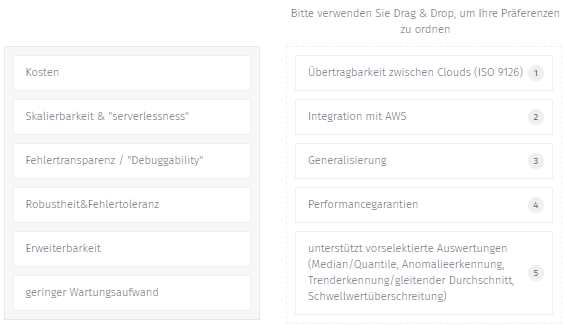
\includegraphics[width=\textwidth]{graphics/Umfrage-Darstellung.png}
\caption{Die Umfrage in QuestionPro}
\label{abb:Umfrage}
\end{figure}


\begin{table}[H]
\centering
\begin{tabular}{|l|l|l|}
\hline
Kriterium & Durchschnitt & gerundet \\ \hline
Übertragbarkeit zwischen Clouds (ISO 9126) & 1,00 & 1 \\ \hline
Integration mit AWS & 3,17 &  3\\ \hline
Generalisierung & 4,33 &  4\\ \hline
Erweiterbarkeit & 4,33 &  4\\ \hline
Fehlertransparenz / \enquote{Debuggability} & 4,67 &  5\\ \hline
geringer Wartungsaufwand & 6,5 &  7\\ \hline
Skalierbarkeit  \& \enquote{serverlessness} & 7,17 &  7\\ \hline
Kosten & 7,33 &  7\\ \hline
Performancegarantien & 8,0 &  8\\ \hline
Robustheit \& Fehlertoleranz & 8,83 &  9\\ \hline
unterstützt Auswertungen (\autoref{chap:auswertungsarten}) & 10,67 & 11 \\ \hlinewd{2pt}
\rowcolor[HTML]{ECF4FF}
Summe & & 66\\ \hline
\end{tabular}
\caption{Auswertungen der Umfragen}
\label{tab:umfragen-auswertungen}
\end{table}

Insgesamt nahmen $n = 6$ Personen teil. Die Ergebnisse sind in \autoref{tab:umfragen-auswertungen} dargestellt.